

\begin{figure}
\centerline{
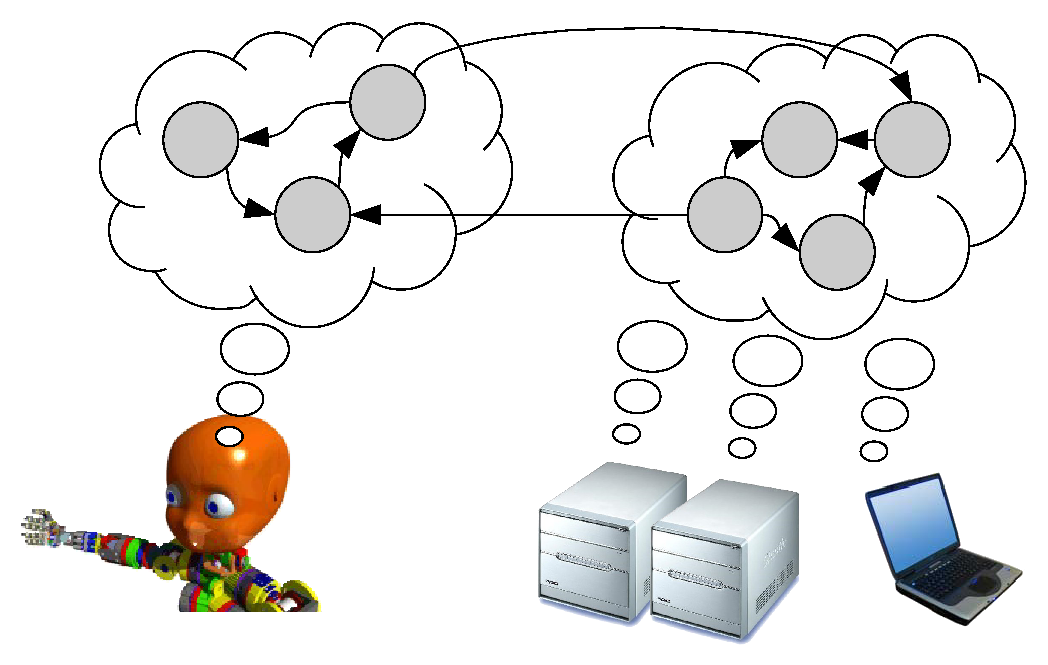
\includegraphics[width=8cm]{fig-nethead}
}
\caption{
%
Basic robot model.  We assume a set of processors, some of which may be
on the robot, some of which may not be.  We assume that the computers
are diverse: they may have different devices, operating systems,
processors, and the programs they run may use different languages,
libraries, etc.  
%
We develop methods for interfacing with devices and communicating
between modules that are useful on any heterogeneous system.
%
We extend our reach by exploiting key Free Software projects
dealing with and enabling diversity in operating systems, build systems, 
and programming languages.
%
Our contribution, made as Free Software, is a system for dealing
with and enabling diversity in transport mechanisms and novel devices.
%
%We nevertheless require that threads within processes
%on any of these computers be able to communicate easily with each other.
%
%This communication, ideally, should fit well with basic UNIX 
%tools and concepts (although we do not assume the operating systems
%in use are UNIX-based).
%
We use this software to support our open robot platform, the iCub
humanoid, whose design will be available under free and open
licensing.
%
}
\end{figure}


\section{Introduction}

%%Hardware defines the environment within which software operates.  

%% Robots can be very unusual software platforms to develop on, perhaps
%% with novel devices or uncommon processors, frequently assembled by a
%% team stronger in mechanical design than computer science.  In fields
%% such as mobile robotics some standardization can be seen, but in
%% humanoids idiosyncracy is the rule.  Can we avoid being a backwater for
%% software development?  We draw lessons from the free software community
%% and UNIX.


Software development is, in some ways, like natural 
evolution.  Every piece of software has its niche:
the environmental conditions within which it can be
used.  Within this niche it will grow and change and 
perhaps expand to nearby niches.
%%
Some niches are very large (for example, commercial PCs), some are
tiny (a newly developed humanoid). Software evolves pretty quickly 
as new technologies get proposed and hardware changes; if trapped 
in a too narrow niche it soon tends to become obsolete and die, 
together with the efforts of the developers who have contributed 
to it. In the academia, software written for a robotic 
project suffer of this plague, because it is rarely written 
by professional developers, and often not the main goal of the 
efforts of the people who are working on it. For researchers 
software development is a time consuming and tedious task that 
takes away time and efforts that could be better spent doing 
research. Yet at the same time, software development in 
robotics is a delicate and crucial task that cannot be easily 
delegated to untrained persons. In research laboratories 
fast changing hardware and lack of human resources too often 
narrow the niche in which software lives.

%
Research to provide intelligence to these complicated robots, perhaps
of humanoid shape, also suffers. Accumulating knowledge 
in the form of working demonstrable systems is plagued by the   
difficulty of forming teams, on agreeing on standards, and in 
general by the lack of a critical mass in any existing laboratory no 
matter the size or funding. The problem of artificial intelligence seems
to be more baffling than what originally thought \ref{} and the year 2006 
celebrated the $50^{th}$ anniversary of the workshop at Dartmouth College
which is unanimously considered the birth of artificial intelligence at 
least in some modern sense \ref{}. %Turing had previously considered the problem%
A generation of researchers did not manage to make the progress that was
certainly hoped for. Significant progress can certainly be made either 
because of a breakthrough in our understanding of the problem or through 
a slower accumulation of knowledge. Or it can be due to a combination of 
these two elements. Recently, the paradigmatic shift toward embodiment 
seems to require also the realization of appropriate robotic hardware \ref{}. 
%Rolf's latest book%
The parallel with the commercial PC is easily made. The success of the PC was
determined, among other factors, by the definition of hardware standards
that everybody could understand, copy, and reimplement. From time
to time new standards were required (e.g. the ISA bus slowly left
space to PCI slots) but the system flourished. A PC of today is the modern 
version of the Theseus' ship, everything changed but the PC is still considered
a PC. 
%
(((the Ship of Theseus -- the mast gets replaced,
the planks get replaced, over time everything may get replaced,
but it is still in some important sense the same ship (``paradox
of identity'').)))
%
Under the hood, the PC is a few orders of magnitude faster and of larger
storage capacity. On the software side, the benefit of a common architecture, 
allowed creating operating systems and application software consisting of 
several millions of lines of code. Without a standard hardware things
might have been more difficult.
It is clearly difficult to foresee the future of humanoid robotics. It is
easier though to imagine a scenario where common standards both in software and
hardware will find the fertile soil to flourish when isolated breakthroughs 
will happen.



Research groups that all use a specific robot (Khepera, Pioneer, AIBO,
...) often form a natural software community.  But each alone is 
a small subset of robotics.

Groups developing new robots face obstacles.  There are big barriers
to software collaboration: differences in sensors, actuators, and
bodies; differences in processors, operating systems, libraries,
frameworks, languages, compilers.


Computer science and PCs operate in a world that has been at least
partially commodified; research groups in CS do not have to 
reinvent the operating system for every project they undertake.


%
In this paper, we are concerned
about how robotics researchers can avoid being caught in a tiny
niche, and how to prevent ``genetic isolation'' from setting in,
where software development is slow and cut-off from the mainstream.
We want to find a way to avoid this trap, without sacrificing
the freedom to radically change our hardware, a freedom that
will be crucial in ``bleeding-edge'' research for years to come.

The only viable solution to these problems is to facilitate 
code reuse both in time and between different people or 
institution. For projects of reasonable size this means following
a \emph{modular} approach, where software is divided in 
independent modules, that can be developed and maintained 
by different people so that efforts 
are shared among groups having distinct competences. A 
modular software platform is flexible. Obsolete modules are 
removed and substituted for newer ones without causing 
catastrophic effects. To take advantage of code written by 
other people in different contexts code must be as friendly 
as possible to other libraries avoiding to impose constraints 
and dependencies at all levels, from the hardware architecture 
to the development environment and programming language. 
Dependencies between modules should be 
minimized also from the point of view of performances; as 
long as resources are available the addition of new 
components should not clash with the existing ones. In 
particular the \emph{timing} of signals should be preserved 
irrespective of the number of modules that are running 
at any given moment in the whole system. 

%
The robotic platform can be seen as another factor on the
equation of code reuse. A common hardware, common protocols,
electrical standards, sensors, etc. can certainly make the 
life of the researchers easier. As for software, modularity 
can play a role in the hardware design too. 

Following the Open Source Software philosophy we make the 
code of our software and hardware available so that other 
researchers can better understand it and have the freedom 
to improve and better adapt it to their needs.

Our motivation comes from the condition of humanoid robotics 
research, but most of this paper is not specific to that field.

%
We think it is relevant to any small research group, either academic or
industrial, who wishes to develop novel robots (as opposed to 
build applications on third party robots).  We want to maximize the 
reach of such research groups. There is clearly a tension here 
between providing a consolidated system and giving enough freedom
to change every single part via upgrades and replacements. We would
like to be able to do so both in software and hardware.


%Robots with unusual hardware can find themselves initially bereft of
%software, until adaptation occurs.  Therefore robots that take
%advantage of novel hardware may require significant software effort.


%Any given piece of software can operate in a certain set of 
%environments.  Every new robot is a new environment, with some
%overlap with existing ones.  Some software will run there,
%some will not.

%In terms of software, robotic platforms can be quite ``genetically
%isolated'' from the mainstream population of PCs.  


%Humanoid robotics is our passion, but in the grand scheme
%of world-wide software development 


%Big companies built on OSS (e.g. Google)

% this might require a few changes to accomodate for the hardware...
New devices come out all the time -- needs to be easy to connect them
to existing code.  YARP needs a minimal ``wrapper'' class to match
vendor-supplied library with relevant interfaces that capture common
capabilities.  YARP encourages separating configuration from source
code -- separating the ``plumbing''.  Devices and communications
remain distinct concerns.  The goal is to allow collaboration between
groups whose robots have different devices and make device changes
less painful.  We also want to have the ability to be able to switch
from remote use of device to local use and vice versa without pain,
without compromising the efficiency of local access.

Robots need an analogue of the operating system of a computer, or the
nervous system of an animal.  We focus on the key issue of how information
travels between processors, sensors, and actuators.

We use other key free and open source projects to make
our libraries usable in as many environments as possible.  We use the
ACE operating system portability layer (but {\it not} the associated
implementation of CORBA), the CMake build system, the SWIG wrapper
generator.

